\documentclass{grattan_pres}\usepackage[]{graphicx}\usepackage[]{color}
%% maxwidth is the original width if it is less than linewidth
%% otherwise use linewidth (to make sure the graphics do not exceed the margin)
\makeatletter
\def\maxwidth{ %
  \ifdim\Gin@nat@width>\linewidth
    \linewidth
  \else
    \Gin@nat@width
  \fi
}
\makeatother

\definecolor{fgcolor}{rgb}{0.345, 0.345, 0.345}
\newcommand{\hlnum}[1]{\textcolor[rgb]{0.686,0.059,0.569}{#1}}%
\newcommand{\hlstr}[1]{\textcolor[rgb]{0.192,0.494,0.8}{#1}}%
\newcommand{\hlcom}[1]{\textcolor[rgb]{0.678,0.584,0.686}{\textit{#1}}}%
\newcommand{\hlopt}[1]{\textcolor[rgb]{0,0,0}{#1}}%
\newcommand{\hlstd}[1]{\textcolor[rgb]{0.345,0.345,0.345}{#1}}%
\newcommand{\hlkwa}[1]{\textcolor[rgb]{0.161,0.373,0.58}{\textbf{#1}}}%
\newcommand{\hlkwb}[1]{\textcolor[rgb]{0.69,0.353,0.396}{#1}}%
\newcommand{\hlkwc}[1]{\textcolor[rgb]{0.333,0.667,0.333}{#1}}%
\newcommand{\hlkwd}[1]{\textcolor[rgb]{0.737,0.353,0.396}{\textbf{#1}}}%
\let\hlipl\hlkwb

\usepackage{framed}
\makeatletter
\newenvironment{kframe}{%
 \def\at@end@of@kframe{}%
 \ifinner\ifhmode%
  \def\at@end@of@kframe{\end{minipage}}%
  \begin{minipage}{\columnwidth}%
 \fi\fi%
 \def\FrameCommand##1{\hskip\@totalleftmargin \hskip-\fboxsep
 \colorbox{shadecolor}{##1}\hskip-\fboxsep
     % There is no \\@totalrightmargin, so:
     \hskip-\linewidth \hskip-\@totalleftmargin \hskip\columnwidth}%
 \MakeFramed {\advance\hsize-\width
   \@totalleftmargin\z@ \linewidth\hsize
   \@setminipage}}%
 {\par\unskip\endMakeFramed%
 \at@end@of@kframe}
\makeatother

\definecolor{shadecolor}{rgb}{.97, .97, .97}
\definecolor{messagecolor}{rgb}{0, 0, 0}
\definecolor{warningcolor}{rgb}{1, 0, 1}
\definecolor{errorcolor}{rgb}{1, 0, 0}
\newenvironment{knitrout}{}{} % an empty environment to be redefined in TeX

\usepackage{alltt}

\title{Working with R}
\author{Hugh Parsonage}
\IfFileExists{upquote.sty}{\usepackage{upquote}}{}
\begin{document}

\begin{frame}{Why use R?}
\begin{enumerate}
\item Free
\item Graphics
\item Programming
\item Reproducibility
\item IDE
\item Packages
\item Community
\end{enumerate}

\end{frame}

\begin{frame}{Why use R?}
\framesubtitle{R is \emph{free}}

Free as in \emph{free beer}:
\begin{itemize}
\item Public can obtain and run your code, with low barrier
\end{itemize}

Free as in \emph{free speech}:
\begin{itemize}
\item You can combine R with other systems, as can commercial entities, without hitting licensing constraints
\item You can inspect and modify the code if you want
\item You know what you are getting
\end{itemize}
\end{frame}

\begin{frame}{Why use R?}
\framesubtitle{R has excellent graphics support}

R's graphics are \emph{publishable}:
\begin{itemize}
\item No need to use external specialist software to produce graphics and charts
\item Data-focused grammar of graphics
\end{itemize}
\end{frame}

\begin{frame}{Why use R?}
\framesubtitle{R is a fully-fledged programming language}

\begin{itemize}
\item Direct, powerful scripted programming 
\item Tasks beyond data, and interacting with external software, can all be achieved from R, in particular \dots{}
\item The way R manages different namespaces and versions is intuitive, simple, and powerful
\end{itemize}
\end{frame}

\begin{frame}{Why use R?}
\framesubtitle{R is fast}
\end{frame}

\begin{frame}{Why use R?}
\framesubtitle{R is the fastest}
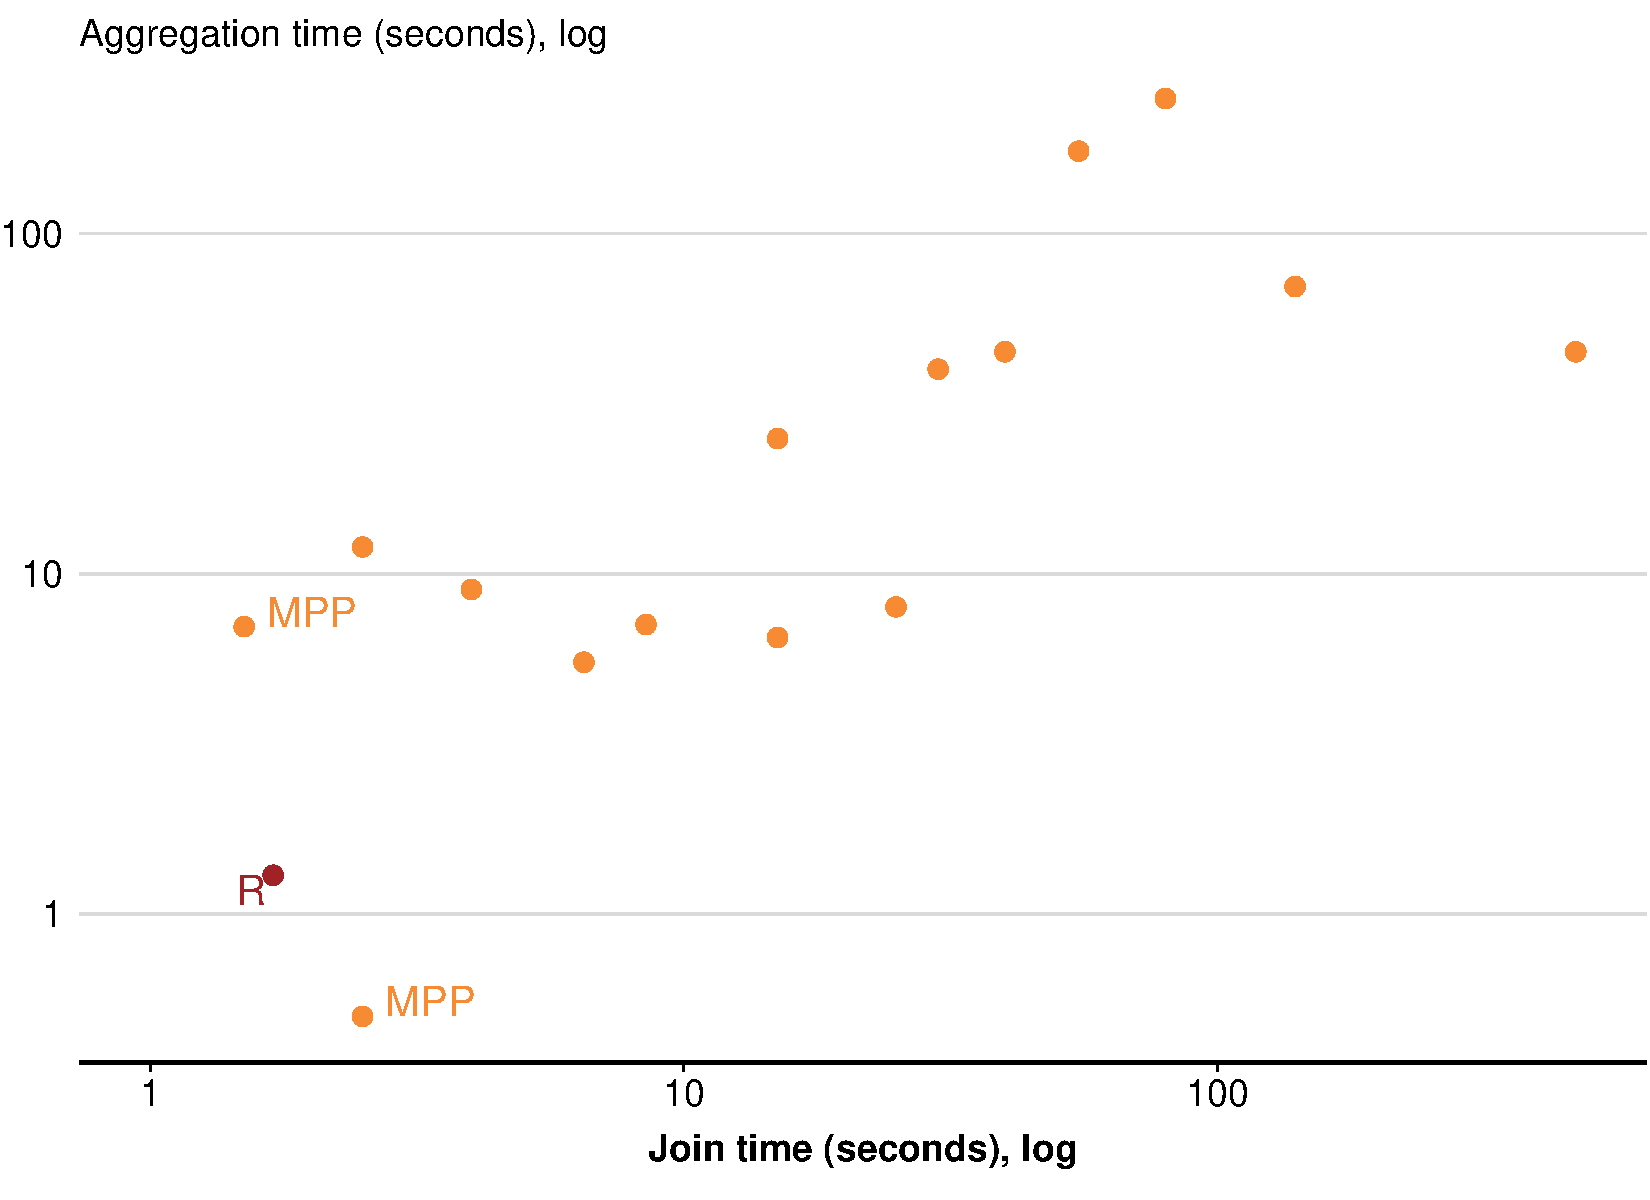
\includegraphics{sziliard-benchmark}
\end{frame}

\begin{frame}{Why use R?}
\framesubtitle{R is the fastest}
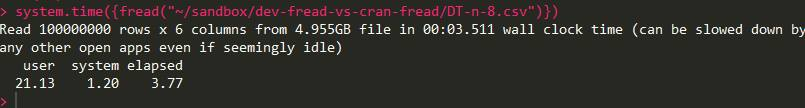
\includegraphics{MattDowle-gone-too-far.jpg}
\end{frame}

\begin{frame}{Why use R?}
\framesubtitle{R makes your work reproducible}
\begin{itemize}
\item[] Never underestimate your ability to make small errors!

\item[] Copying-and-pasting numbers and charts, version control very difficult to do manually.

\item[] R through \texttt{knitr} enables you to embed code, charts, and tables in your document.

\item[] Updates due to new data trivial. \emph{Single-build documents}.
\end{itemize}
\end{frame}

\begin{frame}{Why use R?}
\framesubtitle{IDE}

RStudio, the IDE for R, is excellent.
\end{frame}

\begin{frame}{Why use R?}
\framesubtitle{An outstanding ecosystem of packages}
\begin{itemize}
\item Packages cover literally all statistical tools
\item CRAN is both straightforward to contribute to, easy to access, and maintains a high standard throughout the R community
\end{itemize}
\end{frame}

\begin{frame}{Why use R?}
\framesubtitle{R is well-liked}
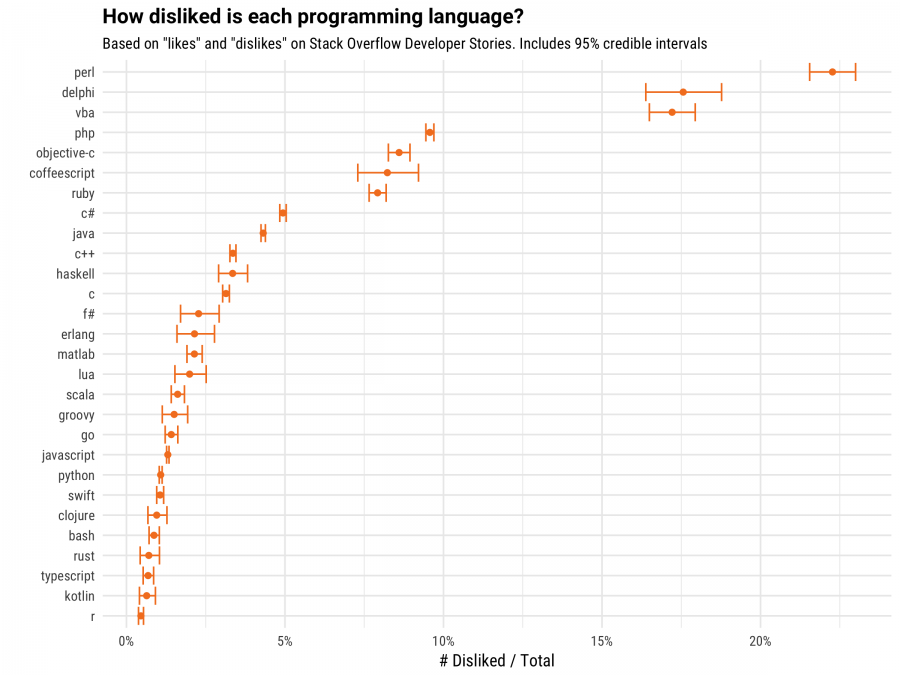
\includegraphics[width=0.8\linewidth]{How-disliked-are-programming-languages-SO}
\source{\url{https://stackoverflow.blog/2017/10/31/disliked-programming-languages/}}
\end{frame}

\begin{frame}{Why use R?}
\framesubtitle{R is growing}
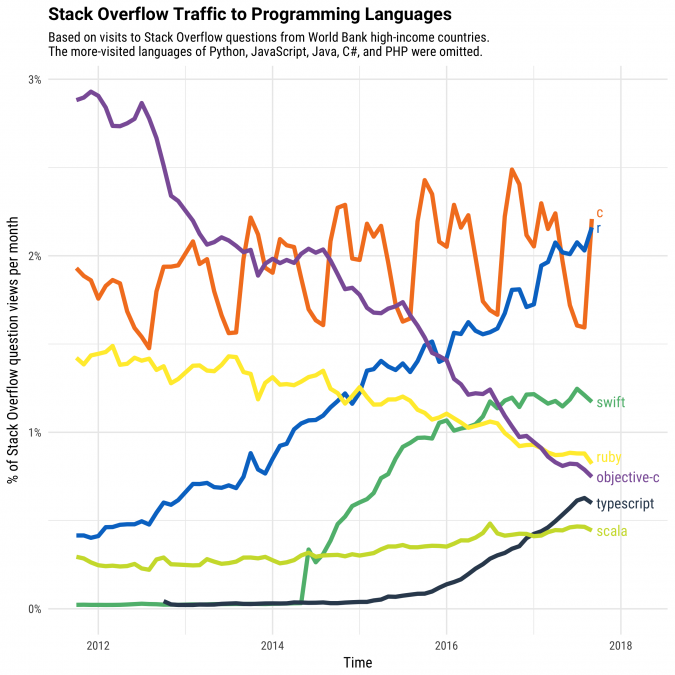
\includegraphics[width=0.7\linewidth]{Growth-of-R}
\source{\url{https://stackoverflow.blog/2017/10/10/impressive-growth-r/}}
\end{frame}

\begin{frame}{Why use R?}
\framesubtitle{Bizarrely good support}
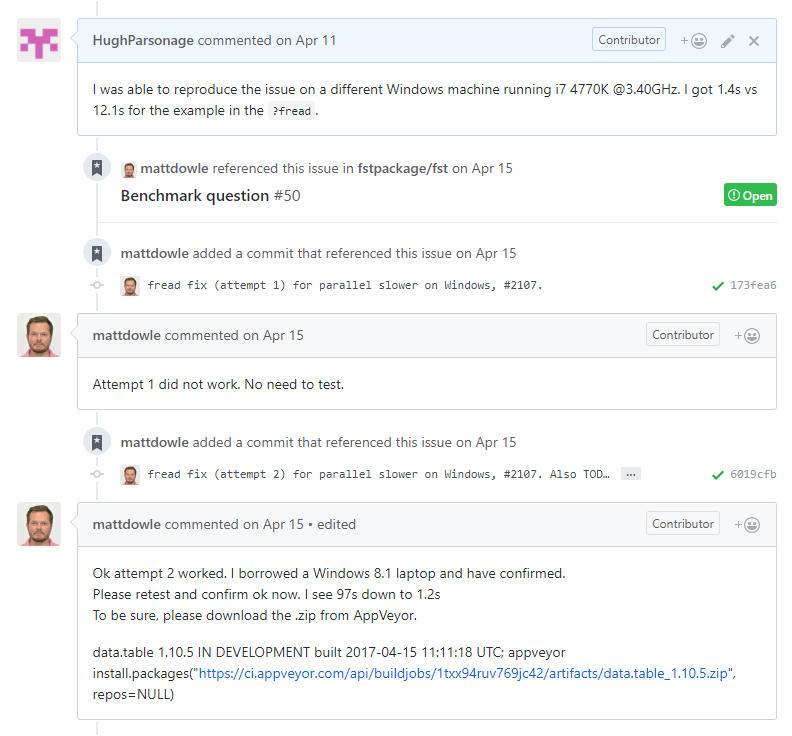
\includegraphics[height=\textheight]{Dowle-support}
\end{frame}






\end{document}
